
\documentclass{article}

%-------------------------------------------------------------------------------------------------------------
%  package
%--------------------------------------------------------------------------------------------------------------
%版面規劃(a4大小,上下左右距0.9inch)
\usepackage[a4paper,margin=0.7in]{geometry}
%作者資訊
\usepackage{authblk}
%中文化package
\usepackage{CJKutf8}


%分兩欄
\usepackage{multicol}
%分欄之後上圖需要有的package
\usepackage{float}
%然後若是需要在其中一欄上面加圖片=>[H大寫]
%要跨欄橫幅的圖片=>{figure*星號要加}[htbp]


%和插入圖片相關的package
\usepackage{graphicx}
\usepackage[tight]{subfigure}
\subfiguretopcaptrue
\usepackage{amsmath,booktabs,threeparttable,url, bm}
%\usepackage[hyphenbreaks]{breakurl}


%連結註腳網頁
\usepackage[colorlinks,linkcolor=blue]{hyperref}



%\newcommand{\cntext}{\begin{CJK}{UTF8}{bsmi}\end{CJK}}

\title{Final Proposal : Solar System \& Interstellar Mission}
\author{Wei-Hsiang Yu 游惟翔}
\affil{Department of Physics, National Tsing Hua University, Hsinchu, Taiwan}

%-------------------------------------------------------------------------------------------------------------
%  文件開始
%--------------------------------------------------------------------------------------------------------------
\begin{document}

\begin{CJK}{UTF8}{bsmi}
%中文化需要加上此行才有title/author/date
\maketitle

\end{CJK}


%摘要(這篇大概在幹嘛)
\begin{abstract}
    This project predicts to improve the solar system simulation based on the program we had done in lecture 7 to make it be able to simulate \textbf{a more real solar system} and use it to find \textbf{trajectories of interstellar probes} that human had launched to the outer space.
\end{abstract}

%開始分兩欄
\begin{multicols}{2}

%-------------------------------------------------------------------------------------------------------------
%  Introduction介紹(大概可以說動機/還有這篇文章的架構/會說些什麼...)
%--------------------------------------------------------------------------------------------------------------
\section{Introduction}

From the class in lecture 7, professor show his program about a n-body system, which can scatter many points in the window, and those object points are projected or even eaten by a star located in the center of the window. I consider that maybe I can simulate one object projected by multiple stars, and that is gravity assist.

So we need a more accurate solar system to acquire a real circumstance for doing simulation, and based on this circumstance and the launched record that some satellites which had launched into the outer space in human history to test this program is exact or not.

There are two satellites will be predicted to simulate in this project: \emph{Voyager2}\cite{b1} \& \emph{Galileo}\cite{b2}. The first one applied gravity assist to speed up over the escape velocity of the Sun, the later one applied gravity assist to speed up for saving the fuel and speed down to make it could be captured by Jupiter.(See Fig.\ref{fig:trajectory})

Finally, if those tests are successful, maybe I will try some other mission's trajectory (like the mission of \emph{Ulysses}, it needed to stop the velocity acquired by launch from earth to 0 but also needed to get the velocity of doing rotation around the Sun to pass the Sun's north and south poles)(See Fig.\ref{fig:tra_u})

% %-------------------------------
\begin{figure*}[htbp]
    \centering
    \subfigure[voyager2]{
        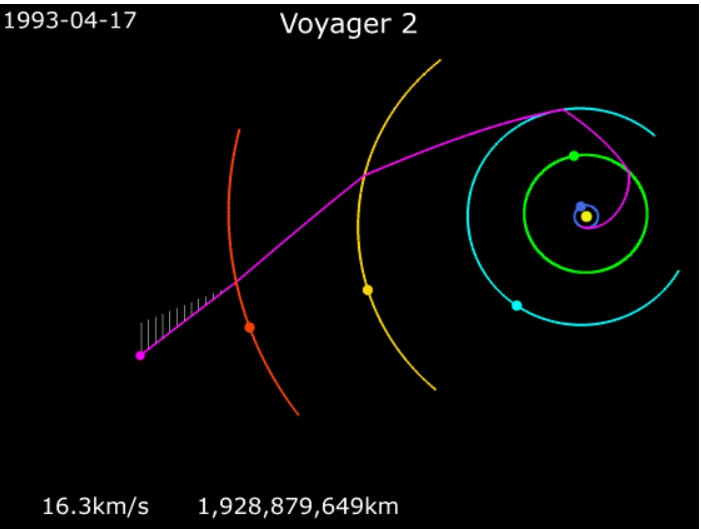
\includegraphics[scale=0.26]{voyager2.jpg}
        \label{fig:tra_v2}
    }
    \subfigure[Galileo]{
        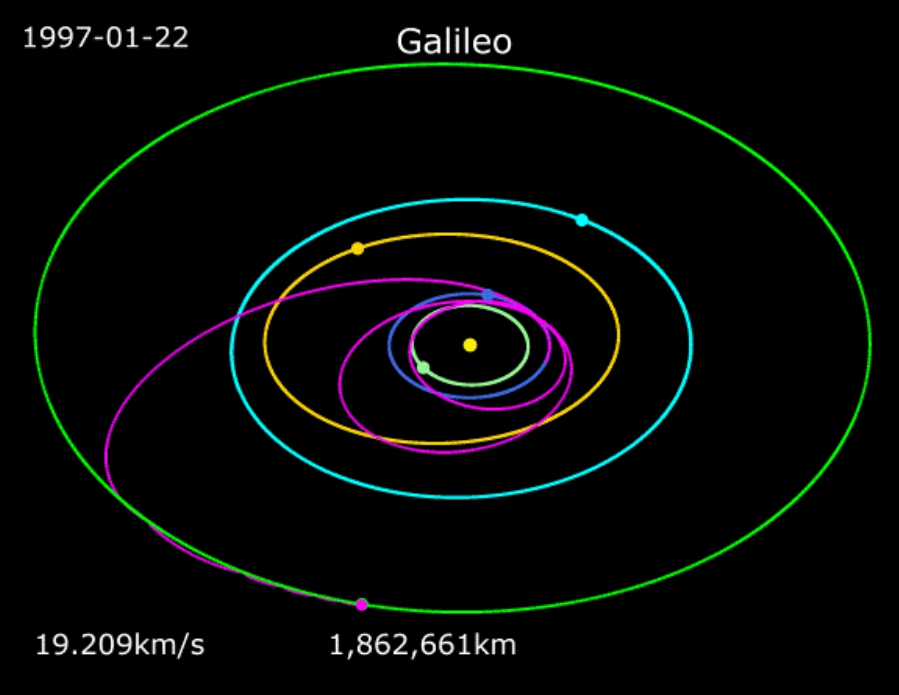
\includegraphics[scale=0.2]{galileo.jpg}
        \label{fig:tra_gali} 
    }
    \subfigure[Ulysses]{
        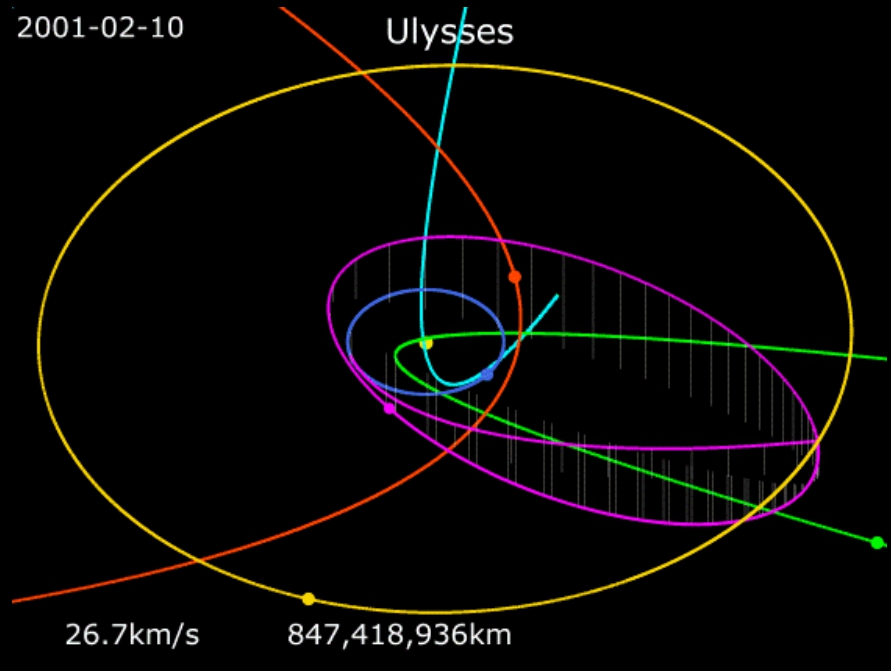
\includegraphics[scale=0.21]{Ulysses.jpg}
        \label{fig:tra_u} 
    }
    \caption{trajectory of three satellite (purple line)}
    \label{fig:trajectory}
\end{figure*}
% %-------------------------------


%-------------------------------------------------------------------------------------------------------------
%  Methodology 方法和細節
%--------------------------------------------------------------------------------------------------------------
\section{Methodology}
There are something need to discuss in this part:
\begin{itemize}
    \item \textbf{Destination} / flyby relay planet of our satellite 
    \item Mechanism for program to \textbf{find trajectories}
    (how it choose or skip this time's trajectory)
\end{itemize}


\subsection{Destination / Flyby Planet / Time}
So, first we need to determine which destination we want to arrive.

\underline{If destination is interstellar}, the velocity of satellite need to over the escape velocity of sun(See Fig.\ref{fig:escape_v}),

% %-------------------------------
\begin{figure}[H]
    \centering 
	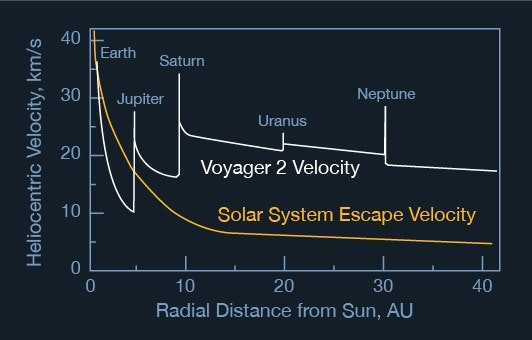
\includegraphics[scale=0.37]{v2_escape.jpeg}
	\caption{The velocity of voyager2 during mission and the escape velocity of the Sun.\cite{b3}} %圖片註解
	\label{fig:escape_v} %label 用這個就可以引用文章當中
\end{figure}
% %-------------------------------

\underline{If the destination is the certain planet}, we need to make our satellite moving as fast as the revolution velocity of the target planet, then our satellite can be captured by the terminal planet.

And we can also record what planet we want to pass (may be pass them to speed up or pass to speed down…)
Choose the time as initial launch time to start our simulation.
Here I think I will start the launch time before the real launch time of voyager2 maybe 1 month before to find that whether this program will get the same result as voyager2 mission report.


\subsection{Instruction Scheme:Find Trajectory}
This part will be the subroutine of the update part in the program done during the class.
Given the initial condition of the launched time coordinate, we then do \textbf{update until the satellite is closed enough the relay planet}.

If the closed enough condition is satisfied, we can then \textbf{use the pass position to determine whether this satellite need to be speed up/speed down} or even will collide with the relay planet. In this part the determination is based on the condition where the destination is. If the destination is the interstellar, we hope that the velocity can increase, but if this planet is the terminal we want to arrive, the determination will hope this flyby being a speed down process.

The tendency of changing velocity is relative to \textbf{how closed the satellite and planet is} and \textbf{where does the satellite pass through the planet}.(See Fig.\ref{fig:speedupdown})

% %-------------------------------
\begin{figure}[H]
    \centering 
	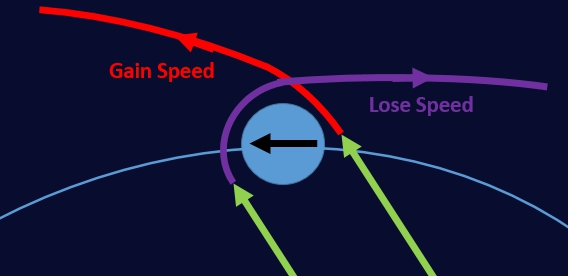
\includegraphics[scale=0.45]{speed_updown.jpg}
	\caption{speed up or speed down} %圖片註解
	\label{fig:speedupdown} %label 用這個就可以引用文章當中
\end{figure}
% %-------------------------------

Above is the steps in one loop, and will recursive update subroutine until the satellite is satisfied with our destination. But there are still some problems need to discuss in this program, and will mention in the next part.

%-------------------------------------------------------------------------------------------------------------
%  Task/Improvement 可以改進的地方
%--------------------------------------------------------------------------------------------------------------
\section{Task \& Improvement}
There are also some tasks will encounter during build this project:

\begin{itemize}
    \item Getting the information of the \textbf{accurate planet coordinate} in special time.
    \item Define \textbf{how close satellite and relay planet}.
    \item Decrease the time of finding the flyby opportunity.
    \item Mechanism of \textbf{adjusting satellite direction} during speeding up or down in gravity assist.
\end{itemize}


\subsection{Accurate Planet Coordinate}
In section 2 we choose a certain time as our satellite initial launch time, but the relative location of each planet in the solar system is required. I found that JPL(Jet Propulsion Laboratory), a institute of NASA, establishing a data base called \textbf{"\emph{horizons}"\cite{b4} to provide a accuracy planet coordinate data} of our solar system from 50 years ago.

This accuracy coordinate data also has \textbf{been sorted out by a Python package "\emph{poliastro}"\cite{b5}} and is able to export to a comprehensible data form.
 
 
\subsection{Define How Close}
During the update part, the condition of how closed the satellite and relay planet is, determinate whether the update do continually or not and the changing tendency of the satellite velocity Respectively.
So a good definition of "closed enough" is a important segment in this program.

This "closed condition" can be considered by the escape velocity generated by each planet the satellite needs to pass.


\subsection{Decrease spending time}
There will be a lot of failures attempts during the update subroutine when our satellite doesn't satisfied the closed condition. Then the loop need to go back to the initial launch time/last departure time and make this time value pulse dt (time+dt) to make another simulation ,but this restart step will consume a lot of time. 

So I may try to define the determination to find how much distance is the satellite and relay planet is, and base on this information to adjust the time interval value. (i.e. making dt become bigger or smaller base on different conditions)


\subsection{Adjusting Direction}
Last thing is given a small adjustment ability of our satellite.
This will be applied when the satellite is coincided with the specified condition of satisfied \textbf{closed enough / pass position}.

By small adjusting direction during gravity assist, we can make the next loop's update become more easier. If the update subroutine fails in the next step, program can first change the adjustment in the last gravity assist instead of restarting the simulation by time+dt.

This task maybe also need to consider the fuel consumption when doing adjustment,
this will influence the update mass during the later time, and change the trajectory.


\end{multicols}

\begin{thebibliography}{00}

\bibitem{b1}
Voyager 2 - Planetary Voyage\\
 \href{https://web.archive.org/web/20131127192310/http://voyager.jpl.nasa.gov/science/planetary.html}{https://web.archive.org/web/20131127192310/http://voyager.jpl.nasa.gov/science/planetary.html}
 
\bibitem{b2}
Galileo - solar system exploration\\
 \href{https://solarsystem.nasa.gov/missions/galileo/overview/}{https://solarsystem.nasa.gov/missions/galileo/overview/}

\bibitem{b3}
Gravity assist: The simple physics trick that’s allowed humanity to explore deep space\\
 \href{https://blog.jatan.space/p/gravity-assist-the-simple-physics-trick-thats-allowed-humanity-to-explore-deep-space}{https://blog.jatan.space/p/gravity-assist-the-simple-physics-trick-thats-allowed-humanity-to-explore-deep-space}

\bibitem{b4}
JPL - horizons\\
 \href{https://ssd.jpl.nasa.gov/horizons.cgi}{https://ssd.jpl.nasa.gov/horizons.cgi}

\bibitem{b5}
Python package - poliastro\\
\href{https://docs.poliastro.space/en/latest/examples/Going\%20to\%20Jupiter\%20with\%20Python\%20using\%20Jupyter\%20and\%20poliastro.html}{https://docs.poliastro.space/en/latest/examples/Going\%20to\%20Jupiter\%20with\%20Python\%20using\\
\%20Jupyter\%20and\%20poliastro.html}

\bibitem{b6}
Gravity\_assist\\
 \href{https://en.wikipedia.org/wiki/Gravity\_assist}{https://en.wikipedia.org/wiki/Gravity\_assist}



\end{thebibliography}

\end{document}

% \footnote{Lagrangian point:\href{https://en.wikipedia.org/wiki/Lagrange\_point}{https://en.wikipedia.org/wiki/Lagrange\_point}}


% %-------------------------------
% \begin{figure}[h]
%     \centering 
% 	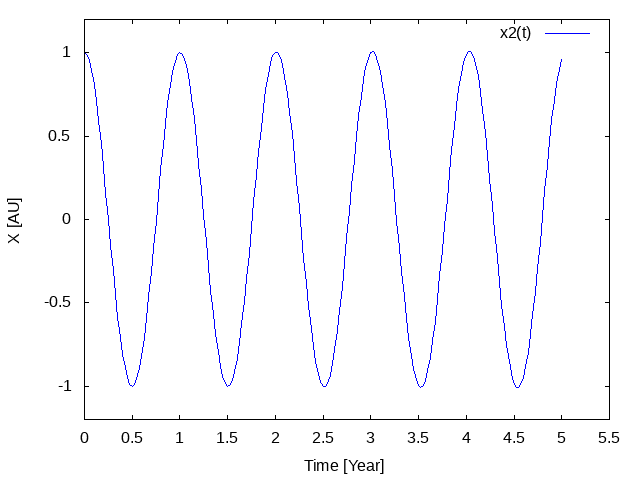
\includegraphics[scale=0.45]{pro1_x2.png}
% 	\caption{The trajectory of $m_1$ $m_2$ (when $m_2$ has a 1.25 factor of velocity).} %圖片註解
% 	\label{fig.pro1} %label 用這個就可以引用文章當中
% \end{figure}
% %-------------------------------

% %-------------------------------
% \begin{figure}[h]
%     \centering
%     \subfigure[dt=0.01yr]{
%         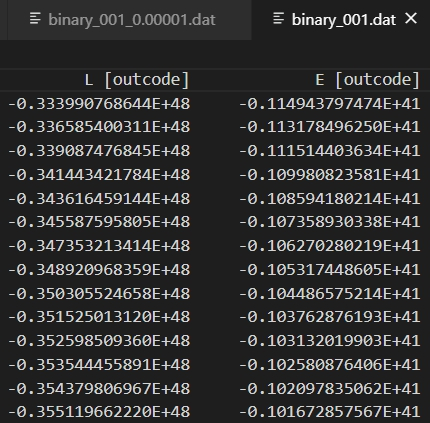
\includegraphics[scale=0.33]{01.jpg}
%         \label{01}
%     }
%     \subfigure[dt=0.001yr]{
%         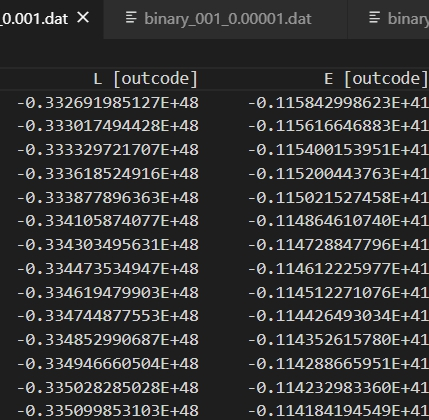
\includegraphics[scale=0.33]{001.jpg}
%         \label{001} 
%     }
%     \subfigure[dt=0.00001yr]{
%         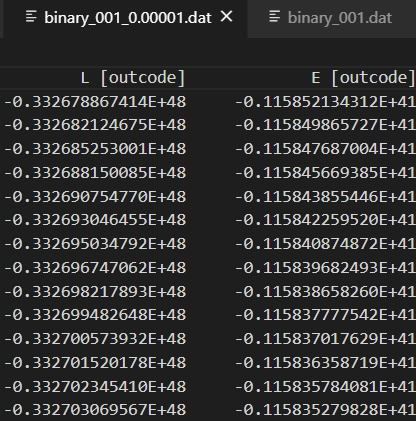
\includegraphics[scale=0.33]{00001.jpg}
%         \label{00001} 
%     }
%     \caption{L \& E in 0.01,0.001,0.00001 time step}
%     \label{fig:2c_dat}
% \end{figure}
% %-------------------------------
